\documentclass[a4paper]{article}

\usepackage[utf8]{inputenc}
\usepackage[T1]{fontenc}
\usepackage[italian]{babel}

\usepackage{graphicx}
\usepackage{siunitx}

\setlength{\marginparwidth}{95pt}

\newcommand*\de{\mathrm{d}}

\title{Relazione laboratorio particelle\\Esperienza 0 (preliminare)}
\author{Andrea Marasciulli\\
Giacomo Petrillo\\
Roberto Ribatti}
\date{Dal 13 al 19 novembre 2017\footnote{Compilazione \LaTeX{} di questo documento: \today.}}

\begin{document}
	
\maketitle

\marginpar{punto 1}

Scegliamo di usare, in ordine dal basso verso l'alto, i PMT 2, 3, 4.

\marginpar{punto 2}

Accendiamo il PMT~2 a \SI{1500}V.

\marginpar{punto 3}

Schizzo dei segnali del PMT visti sull'oscilloscopio:

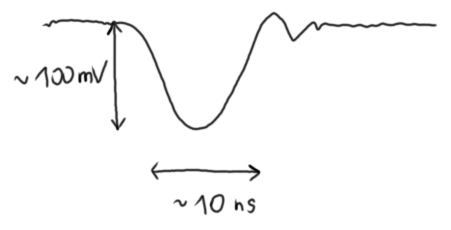
\includegraphics[width=9cm]{fig3a}

Con il trigger a \SI{-27}{mV}, contando a mano su \SI1{min}, otteniamo $\sim\SI1{Hz}$.

\paragraph{Amplificazione}

Stimiamo l'energia rilasciata da una particella nello scintillatore.
Supponiamo MIP, quindi
$\de E/\rho\de x=\SI{1.5}{MeV\,g^{-1}\,cm^2}$.
Lo spessore dello scintillatore è $\sim\SI1\cm$ e la densità $\sim\SI1{g\,cm^{-3}}$,
quindi rilascia $\SI{1.5}{MeV} = \SI{2.4e-13}{J}$.

Stimiamo l'energia del segnale in uscita. È
$\int\de t\, I\cdot V \approx \Delta t\cdot V^2/R$
dove $R=\SI{50}\ohm$, quindi otteniamo
$\num{10e-9}\cdot(\num{100e-3})^2/50=\SI{2e-12}{J}$.

L'amplificazione complessiva è quindi $\sim10$, a naso ce la aspettavamo più grande.

\paragraph{Dipendenza rate dall'alimentazione}

Impostiamo la tensione di alimentazione a \SI{1600}V.
La frequenza di segnali aumenta notevolmente,
per contarli a mano alziamo\footnote{Trattando la logica negativa, useremo alto-basso riferito al modulo e spesso tralasceremo il segno $-$,  la strumentazione suggerisce questo approccio perché la vite della soglia del discriminatore aumenta (abbassa) la soglia in verso orario.} il trigger a \SI{150}{mV},
otteniamo $85/\SI1{min}$.

Con \SI{1800}V otteniamo $\sim\SI{100}{Hz}$ e con \SI{2000}V $\sim\SI{1}{kHz}$
(frequenze misurate dall'oscilloscopio).

\marginpar{punto 4}

\paragraph{Documentazione discriminatore}

Non troviamo la documentazione del nostro discriminatore tra quella fornita;
poiché è a 4 canali e l'unica documentazione per uno a quattro canali è il CAEN~N84,
e inoltre a parte colore e etichette appare identico,
leggiamo la documentazione per quello e chiameremo il nostro <<N84>>.

Documentazione:
ritardo \SI{14}{ns},
durata 6--400\,\si{ns},
soglia massima \SI{400}{mV}.

\paragraph{Verifica discriminatore}

Montiamo questo circuito:

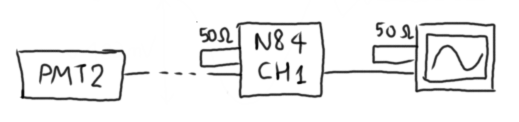
\includegraphics[width=9cm]{fig4a}

Girando la vite della durata vediamo che l'intervallo impostabile è circa 40--300\si{\,ns}.
È di tipo ``restarting'' perché per soglia abbastanza bassa si vedono durate doppie in uscita,
con soglia a opportuni valori intermedi si vedono alternativamente durate doppie oppure due singole, ravvicinate ma non più di tanto.
L'ampiezza è \SI{750}{mV} come atteso.
Verifichiamo la durata impostabile anche per il canale~2, è la stessa.

Modifichiamo il circuito in modo da visualizzare sia l'ingresso che l'uscita del discriminatore:

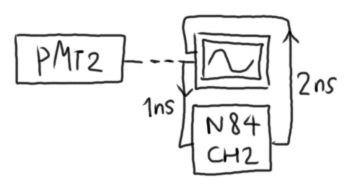
\includegraphics[width=5cm]{fig4b}

Misuriamo la soglia del discriminatore con l'oscilloscopio in questo modo:
triggeriamo sull'ingresso del discriminatore,
se la soglia del discriminatore è minore di quella del trigger
si vede sempre l'uscita del discriminatore,
viceversa a volte scompare.
Trovando due soglie del trigger più vicini possibili in modo che con una a volte scompare l'uscita (verificato su un tempo abbastanza lungo rispetto alla differenza delle soglie) e con l'altra no, si ottiene una misura della soglia del discriminatore.
Il problema di questa procedura è che il trigger dell'oscilloscopio funziona in modo diverso dal discriminatore, quindi non è detto che a parità di soglia vengano selezionati gli stessi segnali.
Con la soglia del discriminatore al massimo otteniamo le soglie del trigger 368 e \SI{376}{mV},
mentre il TP del discriminatore segna \SI{0.411}V, quindi lo scarto è circa \SI8\percent.

Il ritardo è dato da quello dei cavi (\SI3{ns}) più quello del discriminatore.
Puntando i cursori dell'oscilloscopio otteniamo un ritardo di \SI{20}{ns}
quindi il ritardo del discriminatore è circa \SI{17}{ns}.

Ci è difficile misurare il jitter del discriminatore perché il trigger dell'oscilloscopio funziona in modo diverso dal discriminatore, perciò facciamo una stima superiore in questo modo:
mettiamo la soglia del trigger ai \SI{376}{mV} trovati prima che facevano circa coincidere i segnali selezionati, triggerando il segnale del PMT, e guardiamo a occhio sull'oscilloscopio la variazione temporale del fronte di salita dell'uscita del discriminatore; otteniamo \SI{\pm1}{ns}.

\marginpar{punto 5}

\paragraph{Documentazione contatore}

Modello: 130PCZ,
\marginpar{Siamo sicuri o era l'unico datasheet?}%
frequenza massima \SI{70}{MHz},
conta fino a $10^8-1$,
l'input deve durare almeno \SI7{ns},
l'output ``clock'' è un'onda quadra a \SI1{kHz}.
\marginpar{Qual è il duty del clock? \SI{50}\percent?}

\paragraph{Clock del contatore}

Si può collegare il clock all'ingresso~8 per misurare il tempo.
Si può impostare in modo che dopo $10^n$ $(n=2,\dots,8)$
\marginpar{o era $1,\dots,8$?}%
conteggi si fermi.
Se avviamo il conteggio con il pulsante <<start>> o con l'ingresso corrispondente
e lo facciamo fermare in automatico con il clock,
introduciamo un'incertezza sul tempo totale dovuta al non allineamento dello start con il clock\footnote{Potremmo darlo per ovvio, però notiamo che quasi sicuramente i comandi manuali/ingresso non vengono allineati dallo strumento con il fronte successivo del clock perché gli ingressi possono definire intervalli di tempo con molta più granularità di \SI1{ms}.}.
L'incertezza è circa di mezzo periodo, quindi \SI{.5}{ms}.

Visualizziamo il clock sull'oscilloscopio, che calcola una frequenza di \SI{0.99996}{kHz},
cioè la discrepanza è di \SI3s al giorno.
Non sappiamo in che proporzione i due strumenti contribuiscono all'incertezza.
\marginpar{Possiamo fare delle supposizioni?}

\paragraph{Primo test di conteggio}

Montiamo questo circuito:

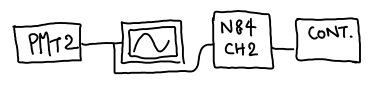
\includegraphics[width=9cm]{fig5a}

Il trigger dell'oscilloscopio è impostato a \SI{376}{mV}.
Mettiamo il clock a 1000 (\SI1s) e facciamo un po' di conteggi.
Il contatore gira intorno a 20;
la frequenza calcolata dall'oscilloscopio oscilla ampiamente perché probabilmente la calcola su intervalli di tempo piccoli rispetto al tasso di conteggi,
quando si stabilizza per qualche secondo gira intorno a \SI{30}{Hz},
quindi non troviamo incongruenze.

\paragraph{Distribuzione dei conteggi}

Ci aspettiamo che, per un tasso costante, i conteggi siano poissoniani con
$\text{media} = \text{tasso}\times \text{tempo}$.
Lo stimatore di massima verosimiglianza per la media è la media aritmetica ed è corretto\footnote{Unbiased.}.
La varianza dello stimatore è la media quindi,
con la convenzione standard di calcolare la varianza nella stima,
per $k$ conteggi il risultato per la media $\mu$ sarà scritto come
\[ \text{<<$\mu = k \pm \sqrt k$>>} \]
Questo è problematico per $k$ piccoli perché la varianza varia velocemente,
risolveremo nell'analisi dati.

\marginpar{punto 6}

\paragraph{Secondo test di conteggio}

Facciamo una serie di conteggi trascrivendo i risultati.
Facciamo 45 conteggi con clock 1000 e 15 con clock \num{10000}.
Verifichiamo che siano poissoniane con un test del $\chi^2$ senza allargare i bin rispetto ai valori discreti;
poiché il numero di conteggi è basso calcoliamo la distribuzione della statistica con monte carlo.
Risultati:

\noindent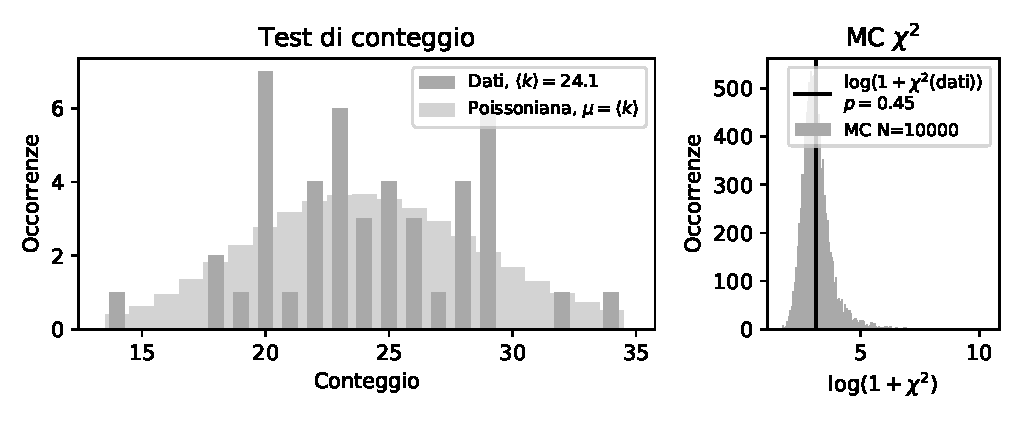
\includegraphics[width=\textwidth]{fig6a}

\noindent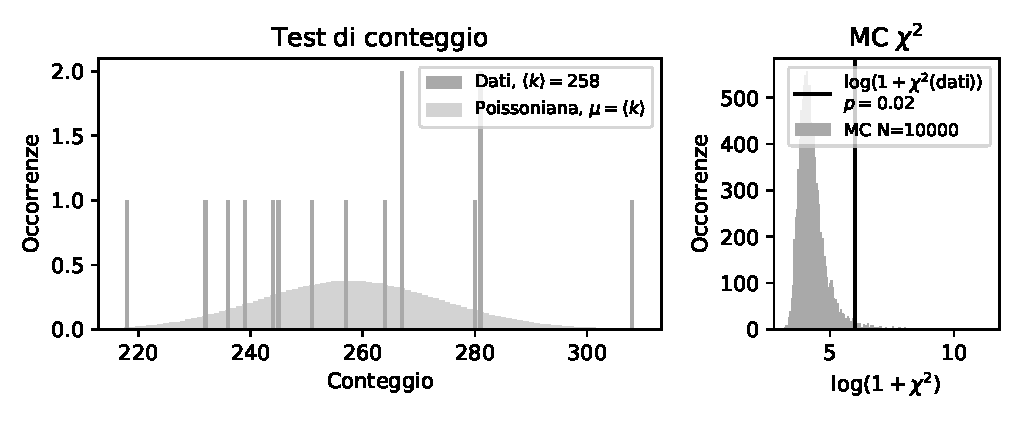
\includegraphics[width=\textwidth]{fig6b}

Vediamo che la poissonianietà della serie da \SI{10}s è in dubbio.

\paragraph{Tempo dall'accensione}

Può darsi che il PMT, dopo l'accensione, ci metta un po' ad arrivare in una condizione stazionaria di funzionamento.
I PMT 3 e 4 li abbiamo lasciati spenti, quindi li usiamo per fare un test.
Accendiamo il PMT~3 e subito prendiamo una serie di 15 conteggi con clock~1000.
Poi accendiamo il PMT~4 e prendiamo una serie, poi proseguiamo alternando PMT~3 e 4,
per un totale di 5 serie. Grafichiamo le medie con la varianza nell'ipotesi di poissoniane:

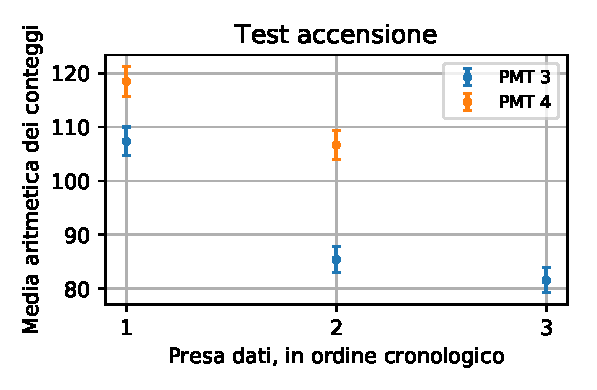
\includegraphics[width=7cm]{fig6c}

Chiaramente il tasso varia nel tempo, quindi in futuro aspetteremo sempre qualche minuto dopo che abbiamo acceso i PMT e almeno 1~minuto quando cambiamo tensione di alimentazione.

\paragraph{Luce ambientale}

Verifichiamo la sensibilità alla luce esterna passando una torcia vicino allo scintillatore e al PMT e verificando se il numero di conteggi cambia sensibilmente.
Testiamo i PMT 2, 3, 4.
\begin{center}
\begin{tabular}{c|p{50ex}}
	PMT & Risultato \\
	\hline
	4 &
	Troviamo un ``buco ottico'' sull'attacco della guida ottica al PMT,
	puntando la torcia i conteggi passano da $\approx 100$ a $\approx 200$. \\
	3 &
	Anche qui l'attacco del PMT alla guida ottica è problematico;
	la luce entra riflettendosi sulla base del PMT.
	I conteggi variano da $\approx 100$ a $\approx 280$.\\
	2 &
	Tutto ok.
\end{tabular}
\end{center}
Sistemiamo tutto con il nastro isolante e ricontrolliamo.

\end{document}
